\documentclass{article}
\usepackage[table, xcdraw]{xcolor}
\usepackage{graphicx}
\usepackage{float}
\usepackage{multirow}
\usepackage{longtable}
\usepackage{array}
\usepackage{listings}
\usepackage{hyperref}

\graphicspath{{images/}}

\hypersetup{
    colorlinks=true,
    linkcolor=blue,
    filecolor=magenta,      
    urlcolor=cyan,
    pdftitle={Overleaf Example},
    pdfpagemode=FullScreen,
    }

\title{Table Layout Regular Expression - Layex}
\author{Romuald Rousseau}
\date{ 2024-03-02 }

\begin{document}

\maketitle

\begin{abstract}
In the modern landscape of data presentation, tables serve as a ubiquitous tool for organizing and conveying information
efficiently. Whether in the structured presentation of scientific findings or the widespread use of spreadsheets in
corporate environments, tables play a pivotal role in facilitating data interpretation. Consequently, the extraction of
valuable insights encapsulated within these tables becomes paramount in any data pipeline process. This white paper
introduces a novel mechanism designed to streamline the extraction of data from tables, particularly those with intricate
layouts. Through the construction of a regular language customized to tabular representation, it aims to enhance efficiency
and accuracy in data extraction processes, ultimately empowering organizations to unlock the full potential of their
tabular data assets.
\end{abstract}

\section{Introduction}
Tables serve as a fundamental tool for organizing and presenting information in a structured and comprehensible manner.
However, the diverse formats and complexities inherent in tables often pose challenges in effectively extracting relevant
data. Recognizing the need for a streamlined solution, this white paper introduces a mechanism designed to decipher the
intricate structures of tables.By offering an efficient method to characterize complex table layouts, this mechanism
enables the accurate detection and extraction of various components and data points. This solution aims to address the
inherent complexities associated with table processing, ultimately enhancing data extraction capabilities for improved
decision-making and analysis. The following figure shows few examples of table layouts:
\begin{figure}[H]
\caption{Various table layouts}
\includegraphics[width=\columnwidth]{various_tables.drawio}
\end{figure}

\section{About other research}
A lot of research is made to extract data from table using machine learning and probabilistic approaches. While those
approaches give very good result, they often failed in the consistence of the results. Our approach is purely
deterministic, therefore the data extraction is very consistent and predictable. To be noted, that our approach can be
used jointly with machine learning, and our compact way to describe table layout can be used to quickly create training
sets and/or labels.

\section{Data Used and Statistics}
The following table shows the number of documents used to experiement and the number od documents that this system since
helped to ingest:
\begin{table}[H]
\centering
\begin{tabular}{|l|l|l|l|}
\hline
Languages & Experiment Docs & Prod Docs  & Prod Records    \\
\hline
8         & 445             & 4,777      & 27,698,600 \\
\hline
\end{tabular}
\end{table}

\section{Anatomy of a table}
By analyzing different layouts based on hundred of documents, a table can be categorized in different basic components:
\begin{itemize}
    \item Columns, Rows, Cells.
    \item Captions, Header, Footer, Body.
    \item Row Groups, Sub-headers, Sub-footers.
\end{itemize}
All these components are structurally linked to each others and form repeated patterns. The basic relation between the
components of a table follows the direction of reading, left top right, top to bottom for most western languages.The
following figure shows a graphical overview of those components and their relation to each others:
\begin{figure}[H]
\caption{Ananomy of a table}
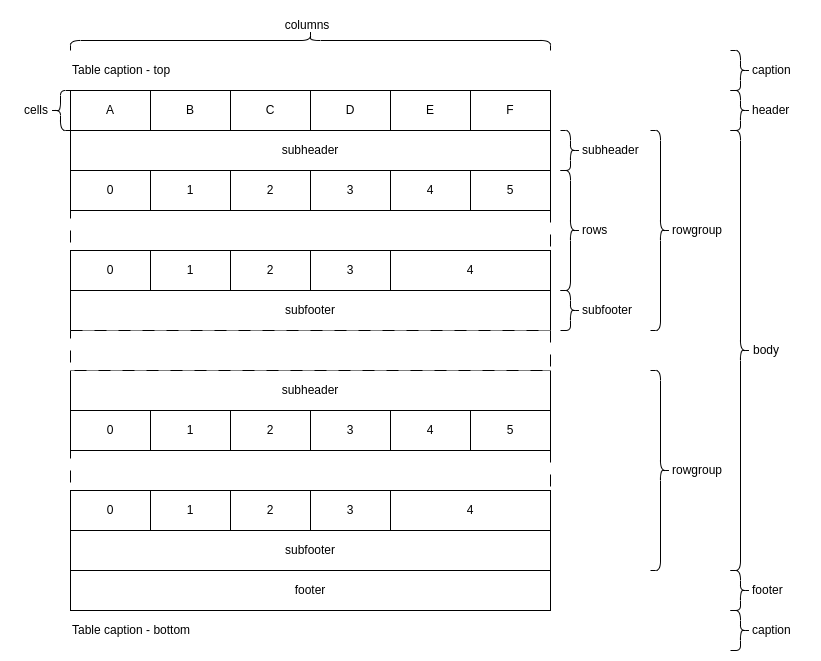
\includegraphics[width=\columnwidth]{table_anatomy.drawio}
\end{figure}

\subsection{More formally}
A table is basically a grid (rows and columns) of cells. Cell is the smallest component of a table. A cell can contain a
value, be empty or be merged with its neighbors. If we look closely, a table can be represented as a stream of cells
ordered through the direction of reading and separated by end of row elements. Below an example of a simple table
represented as a stream of cells, where:
\begin{itemize}
    \item{\$} is an end of row.
    \item{[]} is an empty content of a cell.
    \item{[A-F]} is a content of a header cell.
    \item{[0-5]} is a content of a row cell
\end{itemize}
\begin{figure}[H]
\caption{Stream over a Table}
\includegraphics[width=\columnwidth]{table_stream.drawio}
\end{figure}

\section{Formally}

\subsection{Definition of a Table}
The collection of table T over an alphabet $\Sigma$ is defined recursively as follows:
\begin{itemize}
    \item The empty table Ø is a table
    \item The end of row \$, the singleton $\{\$\}$ is a table
    \item For each cell with a content $c \in \Sigma$, the singleton $\{c\}$ is a table
    \item If A is a table, A* (Kleene star) is a table.
    \item If A and B are tables, then $A \cdot B$ (concatenation) is a table
\end{itemize}

\subsection{Definition of a Reading Direction}
A reading direction is defined by a tuple of a directions. Directions are defined as follows:
\begin{itemize}
    \item Vertical direction when cells are vertically arranged. We can have respectively 2 vertical directions top (T)
    to bottom (B) or bottom (B) to top (T) that we notes respectively TB or BT. 
    \item Horizontal direction when cells are horizontally arranged. We can have respectively 2 horizontal directions
    left (L) to right (R) or right (R) to left (L) that we notes respectively LR or RL. 
    \item The first element of the tuple is the primary direction or line direction and the second element is the
    secondary direction or character direction.
\end{itemize}
Few examples:
\begin{itemize}
    \item TB-LR defines the English direction of reading when we read lines from top to bottom and characters from left
    to right. This direction is sometimes called Gutenberg direction.
    \item TB-RL defines the Arab direction of reading when we read lines from top to bottom and characters from right to
    left
    \item RL-TB defines the traditional Chinese direction of reading when we read lines from right to left and
    characters top to bottom
\end{itemize}

\subsection{Definition of a Stream over a Table and a Reading Direction}
The collection of stream S over the table T and a reading direction R is defined by the following transformations:
\begin{longtable}{|m{0.4\columnwidth}|m{0.3\columnwidth}|m{0.3\columnwidth}|}
\caption{Stream Transformation} \\
% Header    
\hline \rowcolor[HTML]{D0D0D0}
    Reading Direction & Table & Stream \\
\hline
    % Row
    \multirow{2}{*}{TB-LR} & 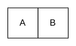
\includegraphics{table-h} & $A \cdot B$ \\
\cline{2-3} 
                           & 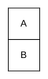
\includegraphics{table-v} & $A \cdot \{\$\} \cdot B$ \\
\hline
    % Row
    \multirow{2}{*}{TB-RL} & 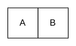
\includegraphics{table-h} & $B \cdot A$ \\
\cline{2-3} 
                           & 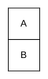
\includegraphics{table-v} & $A \cdot \{\$\} \cdot B$ \\
\hline
    % Row
    \multirow{2}{*}{BT-LR} & 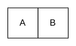
\includegraphics{table-h} & $A \cdot B$ \\
\cline{2-3} 
                           & 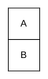
\includegraphics{table-v} & $B \cdot \{\$\} \cdot A$ \\
\hline
    % Row
    \multirow{2}{*}{BT-RL} & 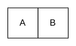
\includegraphics{table-h} & $B \cdot A$ \\
\cline{2-3} 
                           & 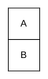
\includegraphics{table-v} & $B \cdot \{\$\} \cdot A$ \\
\hline
    % Row
    \multirow{2}{*}{TB-LR} & 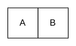
\includegraphics{table-h} & $A \cdot B$ \\
\cline{2-3} 
                           & 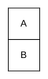
\includegraphics{table-v} & $A \cdot \{\$\} \cdot B$ \\
\hline
    % Row
    \multirow{2}{*}{TB-RL} & 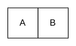
\includegraphics{table-h} & $B \cdot A$ \\
\cline{2-3} 
                           & 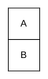
\includegraphics{table-v} & $A \cdot \{\$\} \cdot B$ \\
\hline
    % Row
    \multirow{2}{*}{BT-LR} & 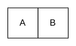
\includegraphics{table-h} & $A \cdot B$ \\
\cline{2-3} 
                           & 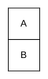
\includegraphics{table-v} & $B \cdot \{\$\} \cdot A$ \\
\hline
    % Row
    \multirow{2}{*}{BT-RL} & 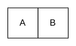
\includegraphics{table-h} & $B \cdot A$ \\
\cline{2-3} 
                           & 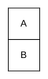
\includegraphics{table-v} & $B \cdot \{\$\} \cdot A$ \\
\hline
\end{longtable}

\subsection{Merged cells}
Cells can be merged with their neighbors however we didn't define this concept in our formalism above. It is because, we
can avoid merged cells by simply copy the content of the cell vertically or horizontally. Formally and depending of the
reading direction:
\begin{itemize}
    \item A cell merged of N cells in the character direction with the content $c \in \Sigma$ can be transformed as a
    concatenation $\{c\}^N$
    \item A cell merged of N cells in the line direction with the content $c \in \Sigma$ can be transformed as a
    concatenation $(\{c\} \cdot \{\$\})^N$
\end{itemize}

\section{Regular Language of a Stream over a Table and a Reading Direction}

\subsection{Regular Language formal definition}
The collection of regular languages over an alphabet $\Sigma$ is defined recursively as follows:
\begin{itemize}
    \item The empty language Ø is a regular language.
    \item For each $a \in \Sigma$(a belongs to $\Sigma$), the singleton language $\{a\}$ is a regular language.
    \item If A is a regular language, A* (Kleene star) is a regular language. Due to this, the empty string language
    $\{\epsilon\}$ is also regular.
    \item If A and B are regular languages, then $A \cup B$ (union) and $A \cdot B$ (concatenation) are regular languages.
    \item No other languages over $\Sigma$ are regular.
\end{itemize}

\subsection{Regular Language of a Stream over a Table and a Reading Direction}
Let define the alphabet $\Sigma = \{s, e, v\}$ as follows:
\begin{itemize}
    \item s, space, is an empty cell (containing spaces or nothing)
    \item e, entity, is a cell containing a string of characters matching a regex $r \in R$
    \begin{itemize}
        \item A number ([0-9]+)
        \item A date ([0-9]{4}-[0-9]{2}-[0-9]{2})
        \item …
    \end{itemize}
\item v, value, is a cell containing a string that is not an entity or a space
\end{itemize}
By construction, a stream over a Table over the alphabet $\Sigma$ and a Reading Direction is a regular language.

\subsection{Regular Expression}
Regular Expression describes a regular language that can be recognized by a finite automaton. A stream over a table and
a reading direction is a regular language and therefore can be describes by a regular expression. It means a regular
expression can match and extract patterns from a table after transformation into a stream over the given table and a
given reading direction.

\section{Table Layout Regular Expression or Layex}
Table Layout Regular Expression or Layex is a syntax implementing a regular expression describing the regular language
of a stream over a table and a reading direction. Layex syntax is similar to the commonly used regex syntax.

\subsection{Boolean "or"}
A vertical bar separates alternatives. For example, gray|grey can match "gray" or "grey".

\subsection{Grouping}
Parentheses are used to define the scope and precedence of the operators (among other uses). For example, gray|grey and
gr(a|e)y are equivalent patterns which both describe the set of "gray" or "grey".

\subsection{Quantification}
A quantifier after an element (such as a token, character, or group) specifies how many times the preceding element is
allowed to repeat. The most common quantifiers are the question mark ?, the asterisk * (derived from the Kleene star),
and the plus sign + (Kleene plus).
\begin{longtable}{|m{0.2\columnwidth}|m{0.8\columnwidth}|}
\caption{Quantification Symbol} \\
    % Header
\hline
    % Row
    ? & The question mark indicates zero or one occurrences of the preceding element. For example, colou?r matches both
    "color" and "colour". \\
\hline
    % Row
    * & The asterisk indicates zero or more occurrences of the preceding element. For example, ab*c matches "ac", "abc",
    "abbc", "abbbc", and so on. \\
\hline
    % Row
    + & The plus sign indicates one or more occurrences of the preceding element. For example, ab+c matches "abc",
    "abbc", "abbbc", and so on, but not "ac". \\
\hline
    % Row
    \{n\} & The preceding item is matched exactly \textit{n} times. \\
\hline
    % Row
    \{min,\} & The preceding item is matched \textit{min} or more times. \\
\hline
    % Row
    \{,max\} & The preceding item is matched up to \textit{max} times. \\
    \hline
    % Row
    \{min,max\} & The preceding item is matched at least \textit{min} times, but not more than \textit{max} times. \\
\hline
\end{longtable}

\subsection{Wildcard}
The wildcard . matches any character. For example, a.b matches any string that contains an "a", and then any character
and then "b". a.*b matches any string that contains an "a", and then the character "b" at some later point.

\subsection{Negation}
The upper case of an element means all but this element; S means everything except space.

\section{General Algorithm}
Below the outline of the algorithm in a pseudo Python language:
\begin{lstlisting}[language=Python, caption=Layex Algorithm]
import re

from openpyxl import load_workbook


def match_entity(v, R):
    for r in R:
    if re.compile(r).match(v) is not None:
        return True
    return False


def cell_to_alphabet(cell, R):
    if cell.value.isspace():
        return "s"
    elif match_entity(cell.value, R):
        return "e"
    else:
        return "v"


def table_to_stream(rows, R):
    for row in rows:
    for cell in row:
        if cell.ismerged():
        for n in cell.merged_horiz_range():
            yield cell_to_alphabet(cell, R)
        else:
        yield cell_to_alphabet(cell, R)
    yield "$"


R = {r'[0-9]'}
reg = re.compile(r'v+$((e|s)+$)+')

wb = load_workbook(
        filename='example.xlsx',
        read_only=True
    )
ws = wb.active

# Supposing re package works on iterable
reg.match(table_to_stream(ws.rows, R))
\end{lstlisting}
Below the basic steps of the algorithm:
\begin{figure}[H]
\caption{Layex Algorithm}
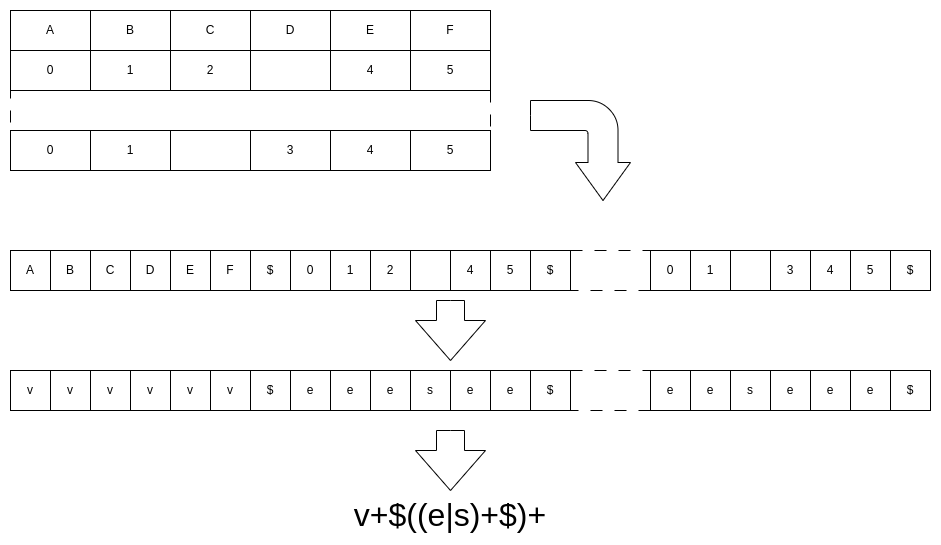
\includegraphics[width=\columnwidth]{layex_algorithm.drawio}
\end{figure}

\section{Results and Statistics}
The following tables give some statitics and the number of layex we wrote to ingest all those documents. The ratio number
of layex verses the quantity of docs parsed demonstrates the flexibility and robusteness of this approach.
\begin{table}[H]
\centering
\begin{tabular}{|l|l|l|}
\hline
Avg Records per Docs & Max Records per Docs  & Layex  \\
\hline
5,798                & 1,048,575             & 15     \\
\hline
\end{tabular}
\end{table}

\section{Few examples}
Layex are a very efficient way to describe complex table layout and therefore detect them and extract the different
components and data from them. Below are few examples.

\subsection{Simple table}
The first example is a simple table with a header and few rows:
\begin{figure}[H]
\caption{Simple Table}
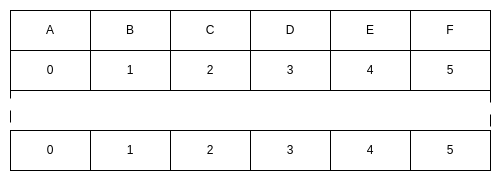
\includegraphics[width=\columnwidth]{simple_table.drawio}
\end{figure}
This simple table can be described with the layex:
\[(.+\$)((.+\$)*)\]
Where,
\begin{itemize}
    \item $(.+\$)$ matches the header
    \begin{itemize}
        \item $((.+\$)*)$ matches the body
        \begin{itemize}
            \item $(.+\$)*$ matches the rows
            \begin{itemize}
                \item $(.+\$)$ matches a row
            \end{itemize}
        \end{itemize}
    \end{itemize}
\end{itemize}

\subsection{Complex table}
The first example is a complex table with a header, sub-header, sub-footer and footer:
\begin{figure}[H]
\caption{Complex Table}
\includegraphics[width=\columnwidth]{complex_table.drawio}
\end{figure}
This simple table can be described with the layex:
\[(v\$)(v+\$)((v\$)(.+\$)*(v\$))*(.+\$)(v\$)\]
Where,
\begin{itemize}
    \item $(v\$)$, matches the top caption
    \item $(v+\$)$ matches the header
    \item $((v\$)(.+\$)*(v\$))*$ matches the body
    \begin{itemize}
        \item $((v\$)(.+\$)*(v\$))$ matches a row-group
        \begin{itemize}
            \item $(v\$)$ matches the sub-header
            \item $(.+\$)*$ matches the rows
            \begin{itemize}
                \item $(.+\$)$ matches a row
            \end{itemize}
            \item $(v\$)$ matches the sub-footer
        \end{itemize}
    \end{itemize}
    \item $(.+\$)$ matches the footer
    \item $(v\$)$ matches the bottom caption
\end{itemize}

\section{References}
\begin{itemize}
    \item \hyperlink{https://en.wikipedia.org/wiki/Regular_expression}{Regular Expression}
    \item \hyperlink{https://www.geeksforgeeks.org/theory-of-computation-automata-tutorials/?ref=lbp}{theory-of-computation-automata-tutorials}
    \item \hyperlink{https://people.cs.umass.edu/~mccallum/papers/TableExtraction-irj06.pdf}{TableExtraction-irj06.pdf}
\end{itemize}

\section{Implementation}

Java - \hyperlink{https://github.com/RomualdRousseau/Any2Json}{github}

\end{document}